\begin{center}\textbf{\color{red}LUYỆN TẬP}\\
	\textbf{CHUYỂN ĐỘNG CỦA VẬT TRONG CHẤT LƯU \\- MOMENT LỰC - ĐIỀU KIỆN CÂN BẰNG}
\end{center}
\section{TRẮC NGHIỆM}
\Opensolutionfile{ans}[ans/D10-KTTX3-BOSUNG]
% ===================================================================
\begin{ex}
	Một ngẫu lực gồm có hai lực $\vec F_1$ và $\vec F_2$, có $F_1 = F_2 = F$ và có cánh tay đòn $d$. Moment ngẫu lực này là	
	\choice
	{$(F_1-F_2)d$}
	{$2Fd$}
	{\True $Fd$}
	{Chưa xác định được}
	\loigiai{}
\end{ex}
% ===================================================================
\begin{ex}
	Cặp lực nào trong hình bên là ngẫu lực?
	\begin{center}
		\includegraphics[scale=0.8]{../figs/D10-KTTX3-BOSUNG-2}
	\end{center}
	\choice
	{Hình a)}
	{\True Hình b)}
	{Hình c)}
	{Hình d)}
	\loigiai{}
\end{ex}
% ===================================================================
\begin{ex}
	Do có khối lượng riêng khoảng \SI{1.29}{\kilogram/\meter^3} nên trọng lượng của không khí gây ra áp suất lên mặt nước biển vào khoảng \SI{101}{\kilo\pascal}. Bề dày của khí quyển Trái Đất được ước lượng bằng
	\choice
	{\SI{7.83}{\meter}}
	{\True \SI{7.83}{\kilo\meter}}
	{\SI{78.3}{\meter}}
	{\SI{78.3}{\kilo\meter}}
	\loigiai{}
\end{ex}
% ===================================================================
\begin{ex}
	Hai lực của ngẫu lực có độ lớn $F=\SI{20}{N}$, khoảng cách giữa hai giá của ngẫu lực là $d=\SI{30}{cm}$. Moment của ngẫu lực có độ lớn bằng
	\choice
	{$\SI{0.6}{\newton\cdot\meter}$}
	{$\SI{600}{\newton\cdot\meter}$}
	{\True $\SI{6}{\newton\cdot\meter}$}
	{$\SI{60}{\newton\cdot\meter}$}
	\loigiai{$$M=Fd = \SI{6}{\newton\cdot\meter}.$$}
\end{ex}
% ===================================================================
\begin{ex}
	Một vật rắn có trục quay cố định, khi tác dụng một lực có độ lớn $\SI{10}{\newton}$ lên vật và khoảng cách từ giá của lực đến trục quay là $\SI{20}{\centi\meter}$ thì moment của lực tác dụng lên vật có độ lớn là $M_1$, khi tác dụng một lực có độ lớn $\SI{15}{\newton}$ lên vật và khoảng cách từ giá của lực đến trục quay là $\SI{5}{\centi\meter}$ thì moment của lực tác dụng lên vật có độ lớn là $M_2$. Chọn hệ thức đúng.
	\choice
	{\True $3M_1=8M_2$}
	{$3M_2=8M_1$}
	{$3M_1=4M_2$}
	{$4M_1=3M_2$}
	\loigiai{}
\end{ex}
% ===================================================================
\begin{ex}
	Cho thanh OB đồng chất có khối lượng $\SI{5}{\kilogram}$ gắn vào tường nhờ bản lề tại O như hình vẽ. Lấy $g=\SI{10}{\meter/\second^2}$. Để thanh OB nằm ngang cân bằng thì cần phải tác dụng vào đầu B một lực hướng lên vuông góc với thanh và có độ lớn bằng
	\begin{center}
		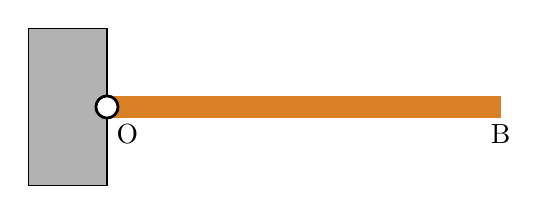
\begin{tikzpicture}
			\coordinate (O) at (0,0);
			\draw[fill=gray!60!white] (0,1) rectangle (-1,-1);
			\draw[line width=8pt, orange!40!brown] (0,0)--(5,0);
			\draw[line width=1pt, fill=white] (0,0) circle(4pt);
			\node[below right] at (0,-0.1) {O};
			\node[below] at (5,-0.1) {B};
		\end{tikzpicture}
	\end{center}
	\choice
	{$\SI{15}{\newton}$}
	{\True $\SI{25}{\newton}$}
	{$\SI{10}{\newton}$}
	{$\SI{30}{\newton}$}
	\loigiai{}
\end{ex}
% ===================================================================
\begin{ex}
	Một thanh đồng chất có chiều dài $L$, trọng lượng $\SI{200}{\newton}$, treo một vật có trọng lượng $\SI{450}{\newton}$ vào thanh như hình \ref{fig:23.5}. Các lực $\vec F_1$, $\vec F_2$ của thanh tác dụng lên hai điểm tựa có độ lớn lần lượt là
	\begin{center}
		\includegraphics[width=0.4\linewidth]{../figs/VN10-2022-PH-TP023-P-5}
		\captionof{figure}{}
		\label{fig:23.5}
	\end{center}
	\choice
	{\True $\SI{212.5}{\newton}$; $\SI{437.5}{\newton}$}
	{$\SI{325}{\newton}$; $\SI{325}{\newton}$}
	{$\SI{437.5}{\newton}$; $\SI{212.5}{\newton}$}
	{$\SI{487.5}{\newton}$; $\SI{162.5}{\newton}$}
	\loigiai{Các lực thành phần theo phương $Oy$ cân bằng nhau:
		\begin{equation}
			\label{eq:23.1}
			F_1+F_2-200-450=0
		\end{equation}
		Áp dụng quy tắc moment lực đối với trục quay tại A:
		\begin{equation}
			\label{eq:23.2}
			\dfrac{L}{2}\cdot 200+\dfrac{3L}{4}\cdot 450=LF_2
		\end{equation}
		Từ (\ref{eq:23.1}) và (\ref{eq:23.2}), suy ra $F_1=\SI{212.5}{\newton}$, $F_2=\SI{437.5}{\newton}$.}
\end{ex}
% ===================================================================
\begin{ex}
	Đòn bẩy có cấu tạo như hình \ref{fig:0005-1}. Đầu A của đòn bẩy treo một vật có trọng lượng $\SI{30}{\newton}$. Chiều dài đòn bẩy dài $\SI{50}{\centi\meter}$. Khoảng cách từ đầu A đến trục quay O là $\SI{20}{\centi\meter}$. Cần phải treo một vật khác có trọng lượng bằng bao nhiêu ở đầu B để đòn bẩy cân bằng?
	\begin{center}
		\includegraphics[width=0.35\linewidth]{../figs/VN10-2023-PH-TP0005-1}
		\captionof{figure}{}
		\label{fig:0005-1}
	\end{center}	
	\choice
	{$\SI{15}{\newton}$}
	{\True $\SI{20}{\newton}$}
	{$\SI{25}{\newton}$}
	{$\SI{30}{\newton}$}
	\loigiai{Áp dụng quy tắc moment với trục quay qua O:
		$$P_\text{A}\cdot OA=P_\text{B}\cdot OB\Rightarrow P_\text{B}=\dfrac{P_\text{A}\cdot OA}{OB}=\dfrac{\left(\SI{30}{\newton}\right)\cdot\left(\SI{20}{\centi\meter}\right)}{\SI{30}{\centi\meter}}=\SI{20}{\newton}.$$}
\end{ex}
% ===================================================================
\begin{ex}
	Một đường ống đồng chất có trọng lượng $\SI{100}{\newton}$, chiều dài $L$, tựa trên điểm tựa như hình \ref{fig:23.3}. Khoảng cách $x$ và độ lớn phản lực $F_R$ của điểm tựa tác dụng lên đường ống là
	\begin{center}
		\includegraphics[width=0.4\linewidth]{../figs/VN10-2022-PH-TP023-P-3}
		\captionof{figure}{}
		\label{fig:23.3}
	\end{center}	
	\choice
	{\True $x=0,69L$; $F_R=\SI{800}{\newton}$}
	{$x=0,69L$; $F_R=\SI{400}{\newton}$}
	{$x=0,6L$; $F_R=\SI{552}{\newton}$}
	{$x=0,6L$; $F_R=\SI{248}{\newton}$}
	\loigiai{Áp dụng quy tắc moment lực đối với trục quay tại A:
		\begin{center}
			\includegraphics[width=0.4\linewidth]{../figs/VN10-2022-PH-TP023-P-4}
		\end{center}
		$$x\cdot 200+\left(x-\dfrac{L}{2}\right)\cdot100=\left(L-x\right)\cdot500$$
		$$\Rightarrow x=0,69L$$
		Các lực thành phần theo phương $Oy$:
		$$F_R-200-100-500=0\Rightarrow F_R=\SI{800}{\newton}.$$}
\end{ex}
% ===================================================================
\begin{ex}
	Một tấm ván nặng $\SI{270}{\newton}$ được bắc qua một con mương. Trọng tâm của tấm ván cách điểm tựa trái $\SI{0.8}{\meter}$ và cách điểm tựa phải là $\SI{1.6}{\meter}$. Hỏi lực mà tấm ván tác dụng lên điểm tựa bên trái có độ lớn là bao nhiêu?	
	\choice
	{\True $\SI{180}{\newton}$}
	{$\SI{90}{\newton}$}
	{$\SI{160}{\newton}$}
	{$\SI{80}{\newton}$}
	\loigiai{\begin{center}
			\includegraphics[width=0.4\linewidth]{../figs/VN10-2022-PH-TP023-P-2}
		\end{center}
		Áp dụng quy tắc moment cho trục quay qua điểm tựa phải:
		$$P\cdot d_2=F'_1\cdot\left(d_1+d_2\right)$$
		với $\vec F'_1=-\vec F_1$ là lực do điểm tựa trái tác dụng lên ván.
		$$\Rightarrow F'_1=\dfrac{P\cdot d_2}{d_1+d_2}=\SI{180}{\newton}$$
		Lực do ván tác dụng lên điểm tựa trái:
		$$F_1=F'_1=\SI{180}{\newton}.$$}
\end{ex}
% ===================================================================
\begin{ex}
	Thanh nhẹ OB có thể quay quanh trục O. Tác dụng lên thanh các lực $F_1$ và $F_2$ đặt tại B và A. Biết lực $F_1=\SI{20}{\newton}$, $OA=\SI{10}{\centi\meter}$, $AB=\SI{40}{\centi\meter}$. Thanh cân bằng, các lực $F_1$ và $F_2$ hợp với AB các góc $\alpha=\SI{30}{\degree}$, $\beta=\SI{90}{\degree}$. Độ lớn lực $F_2$ là
	\begin{center}
		\includegraphics[width=0.25\linewidth]{../figs/VN10-2023-PH-TP0005-8}
	\end{center}
	\choice
	{$\SI{100}{\newton}$}
	{\True $\SI{50}{\newton}$}
	{$\SI{200}{\newton}$}
	{$\xsi{\dfrac{100}{\sqrt{3}}}{\newton}$}
	\loigiai{Áp dụng quy tắc moment với điểm tựa O:
		$$F_1d_1=F_2d_2\Leftrightarrow F_1\cdot OB\sin\SI{30}{\degree}=F_2\cdot OA \Rightarrow F_2=\dfrac{F_1\cdot OB\sin\SI{30}{\degree}}{OA}=\SI{50}{\newton}.$$}
\end{ex}
% ===================================================================
\begin{ex}
	Một người dùng búa để nhổ một chiếc đinh. Khi người ấy tác dụng một lực $F=\SI{100}{\newton}$ vào đầu búa thì đinh bắt đầu chuyển động. Lực cản của gỗ tác dụng vào đinh bằng
	\begin{center}
		\includegraphics[width=0.15\linewidth]{../figs/VN10-2023-PH-TP0005-2}
	\end{center}	
	\choice
	{$\SI{500}{\newton}$}
	{\True $\SI{1000}{\newton}$}
	{$\SI{1500}{\newton}$}
	{$\SI{2000}{\newton}$}
	\loigiai{\begin{center}
			\includegraphics[width=0.15\linewidth]{{../figs/VN10-2023-PH-TP0005-3}}
		\end{center}
		Áp dụng quy tắc moment với trục quay qua điểm tựa của đầu búa với đất:
		$$F\cdot\left(\SI{20}{\centi\meter}\right)=F_c\cdot\left(\SI{2}{\centi\meter}\right)\Rightarrow F_c=10F=\SI{1000}{\newton}.$$}
\end{ex}
% ===================================================================
\begin{ex}
	Một người nâng một tấm gỗ đồng chất, tiết diện đều, có trọng lượng $P=\SI{200}{\newton}$. Người ấy tác dụng một lực $\vec F$ thẳng đứng lên phía trên vào đầu trên của tấm gỗ để giữ cho nó hợp với mặt đất một góc $\alpha=\SI{30}{\degree}$. Độ lớn lực $F$ bằng	
	\begin{center}
		\includegraphics[width=0.25\linewidth]{../figs/VN10-2023-PH-TP0005-5}
	\end{center}
	\choice
	{\True $\SI{100}{\newton}$}
	{$\SI{86.6}{\newton}$}
	{$\SI{50}{\newton}$}
	{$\SI{50.6}{\newton}$}
	\loigiai{Áp dụng quy tắc moment với điểm tựa là đầu thanh gắn với đất:
		$$P\cdot\dfrac{\ell}{2}\cos\SI{30}{\degree}=F\cdot\ell\cos\SI{30}{\degree}\Rightarrow F=\dfrac{P}{2}=\SI{100}{\newton}.$$}
\end{ex}
% ===================================================================
\begin{ex}
	Một người nâng một tấm gỗ đồng chất, tiết diện đều, có trọng lượng $P=\SI{200}{\newton}$. Người ấy tác dụng một lực $F$ vào đầu trên của tấm gỗ (vuông góc với tấm gỗ) để giữ cho nó hợp với mặt đất một góc $\alpha=\SI{30}{\degree}$. Độ lớn lực $F$ bằng 
	\begin{center}
		\includegraphics[width=0.25\linewidth]{../figs/VN10-2023-PH-TP0005-6}
	\end{center}
	\choice
	{$\SI{100}{\newton}$}
	{$\SI{50}{\newton}$}
	{\True $\SI{86.6}{\newton}$}
	{$\SI{50.6}{\newton}$}
	\loigiai{Áp dụng quy tắc moment với điểm tựa tại đầu thanh chạm đất:
		$$P\cdot\dfrac{\ell}{2}\cos\SI{30}{\degree}=F\cdot\ell\Rightarrow F=\dfrac{P}{2}\cdot\cos\SI{30}{\degree}=\SI{86.6}{\newton}.$$}
\end{ex}
% ===================================================================
\begin{ex}
	Một vật rắn phẳng, mỏng, dạng tam giác đều ABC, cạnh $a=\SI{20}{\centi\meter}$. Người ta tác dụng vào một ngẫu lực nằm trong mặt phẳng của tam giác. Các lực có độ lớn $\SI{8}{\newton}$ và đặt vào hai đỉnh A và C, song song với BC. Moment của ngẫu lực có độ lớn là
	\choice
	{$\SI{13.8}{\newton\cdot\meter}$}
	{\True $\SI{1.38}{\newton\cdot\meter}$}
	{$\SI{13.8E-2}{\newton\cdot\meter}$}
	{$\SI{13.8E-3}{\newton\cdot\meter}$}
	\loigiai{Cánh tay đòn ngẫu lực chính bằng đường cao kẻ từ A của tam giác ABC:
		$$d=AH=\dfrac{a\sqrt{3}}{2}=\xsi{10\sqrt{3}}{\centi\meter}$$
		Moment của ngẫu lực:
		$$M=Fd=\left(\SI{8}{\newton}\right)\cdot\left(\xsi{0,1\sqrt{3}}{\meter}\right)=\SI{1.38}{\newton\cdot\meter}.$$}
\end{ex}
\Closesolutionfile{ans}
\section{BÀI TẬP TỰ LUẬN}
\setcounter{ex}{0}
% ======================================================================
\begin{ex}
	\immini{Một xe cẩu có chiều dài cần trục $\ell=\SI{20}{\meter}$ và nghiêng góc $\SI{30}{\degree}$ so với phương thẳng đứng. Đầu cần trục có treo một thùng hàng nặng 2 tấn như hình bên. Xác định moment lực do thùng hàng tác dụng lên đầu cần trục đối với trục quay đi qua đầu còn lại của cần trục gắn với thân máy. Lấy $g=\SI{9.8}{\meter/\second^2}$.}
	{\vspace{-1cm}\includegraphics[scale=0.65]{../figs/D10-KTTX3-BOSUNG-5}}
	\loigiai{$M=F\ell\sin\SI{30}{\degree}=\SI{196}{\kilo\newton\cdot\meter}$.}
\end{ex}
% ======================================================================
\begin{ex}
	\immini{Một bình hình chữ U chứa các chất lỏng A và B không hòa tan, không phản ứng với nhau sẽ có trạng thái ổn định như hình bên. Thước đo gắn với bình có đơn vị đo là $\si{\centi\meter}$.
		\begin{enumerate}[label=\alph*)]
			\item Nhận xét về áp suất tại các điểm thuộc hai nhánh ống nhưng đều ở mực chất lỏng $L$?
			\item So sánh khối lượng riêng của hai chất lỏng A và B.
	\end{enumerate}}
	{\vspace{-0.75cm}\includegraphics[scale=0.5]{../figs/D10-KTTX3-BOSUNG-1}}
	\loigiai{
	\begin{enumerate}[label=\alph*)]
		\item Áp suất tại hai điểm nằm cùng trên mặt ngang trong lòng chất lỏng là như nhau.
		\item Xét các điểm thuộc hai nhánh ống nằm ở mực chất lỏng M như hình bên sẽ có cùng áp suất, tức là:
		$$\rho_{\mathrm{B}}gh_{\mathrm{B}}=\rho_{\mathrm{A}}gh_{\mathrm{A}}\Rightarrow\dfrac{\rho_{\mathrm{A}}}{\rho_{\mathrm{B}}}=\dfrac{h_{\mathrm{B}}}{h_{\mathrm{A}}}=\dfrac{50}{60}=\dfrac{5}{6}.$$
	\end{enumerate}
	}
\end{ex}
% ======================================================================
\begin{ex}
	\immini{Một quả cầu có trọng lượng $P=\SI{40}{\newton}$ được treo vào tường nhờ một sợi dây hợp với mặt tường một góc $\alpha=\SI{30}{\degree}$. Bỏ qua ma sát ở chỗ tiếp xúc giữa quả cầu và tường. Xác định:
		\begin{enumerate}[label=\alph*)]
			\item lực căng dây treo.
			\item phản lực của tường tác dụng lên quả cầu.
	\end{enumerate}}
	{\vspace{-0.75cm}\includegraphics[scale=0.8]{../figs/D10-KTTX3-BOSUNG-4}}
	\loigiai{$T=\dfrac{P}{\cos\SI{30}{\degree}}\approx\SI{46.2}{\newton}$, $N=P\tan\SI{30}{\degree}\approx\SI{23.09}{\newton}$.}
\end{ex}
% ======================================================================
\begin{ex}
	Thanh AB khối lượng $m$, chiều dài $L=\SI{3}{\meter}$ gắn vào tường với bản lề A. Đầu B của thanh treo vật nặng $\SI{5}{\kilogram}$. Thanh được giữ nằm ngang nhờ dây treo CD, biết lực căng dây $\SI{150}{\newton}$, $\mathrm{AC}=\SI{2}{\meter}$, dây treo hợp với thanh AB một góc $\alpha=\SI{45}{\degree}$ như hình vẽ bên dưới. 
	\begin{center}
		\includegraphics[width=0.25\linewidth]{../figs/VN10-2022-PH-TP023-P-11}
	\end{center}
	Xác định moment của lực căng dây CD và moment lực căng dây ở đầu B đối với trục quay qua A. Lấy $g=\SI{10}{\meter/\second^2}$.	
	\loigiai{
		Moment của lực căng dây:
		$M_{T_{\mathrm{B}/\mathrm{A}}}=T_{\mathrm{B}}\cdot\mathrm{AB}=m_{\mathrm{B}}g\cdot\mathrm{AB}=\SI{150}{\newton\meter}$.
		\\
		$M_{T_{\mathrm{CD}/\mathrm{A}}}=T_{\mathrm{CD}}\cdot\mathrm{AC}\sin\alpha=\xsi{150\sqrt{2}}{\newton\meter}$.
	}
\end{ex}
% ======================================================================
\begin{ex}
	Một chiếc thước mảnh có trục quay nằm ngang đi qua trọng tâm O của thước. Dùng hai ngón tay tác dụng vào thước một ngẫu lực đặt vào hai điểm A và B cách nhau $\SI{4.5}{\centi\meter}$ và có độ lớn $F_{\mathrm{A}}=F_{\mathrm{B}}=\SI{1}{\newton}$.
	Thước quay đi một góc $\alpha=\SI{30}{\degree}$. Hai lực luôn luôn nằm ngang và vẫn đặt tại A và B (hình vẽ). Tính moment ngẫu lực lúc bấy giờ.
	\begin{center}
		\begin{tikzpicture}
			\coordinate (O) at (0,0);
			\coordinate (A) at ($(O)+(60:2)$);
			\coordinate (B) at ($(O)+(-120:2)$);
			\coordinate (FA) at ($(A)+(2,0)$);
			\coordinate (FB) at ($(B)+(-2,0)$);
			\coordinate (I) at ($(B)+(90:3.4641)$);
			\tkzMarkAngle[size=0.75cm,color=red, line width=1pt](A,B,I);
			\node [draw, thick, shape=rectangle, minimum width=0.3cm, minimum height=4.5cm, anchor=center, fill=gray!40!white, rotate=-30] at (O) {};
			\fill   (O) circle[radius=2pt]  node [right] {};
			\draw[line width=2pt, -stealth, line width=2pt, blue] (A)--(FA);
			\draw[line width=2pt, -stealth, line width=2pt, blue] (B)--(FB);
			\draw[dashed, line width=1pt] (B)--(I)--(A);
			\draw[dashed, line width=1pt] (0,-2)--(0,2);
			\node[right] at ($(B)+(0.2,0)$) {B};
			\node[above left] at ($(A)+(-0.2,0)$) {A};
			\node[right] at ($(O)+(0.2,0)$) {O};
			\node[above] at (I) {I};
			\node[above] at (FA) {$\vec{F}_{\mathrm{A}}$};
			\node[above] at (FB) {$\vec{F}_{\mathrm{B}}$};
			
			\tkzLabelAngle[color=black,pos=1.2](A,B,I){$\alpha$};
		\end{tikzpicture}
	\end{center}
	\loigiai{$M=F\cdot \mathrm{BI}=F\cdot \mathrm{AB}\cos\alpha\approx\SI{0.039}{\newton\cdot\meter}$.}
\end{ex}
% ======================================================================
\begin{ex}
	\immini{Một thanh dài AO, đồng chất, tiết diện đều, có khối lượng \SI{1.2}{\kilogram}. Một đầu O của thanh liên kết với tường bằng một bản lề, còn đầu A được treo vào tường bằng một sợi dây AB. Thanh được giữ nằm ngang và dây làm với thanh một góc $\alpha=\SI{30}{\degree}$. Lấy $g=\SI{10}{\meter/\second^2}$. Tính lực căng của dây.}
	{\includegraphics[scale=0.7]{../figs/D10-KTTX3-BOSUNG-3}}
	\loigiai{
	Áp dụng quy tắc moment đối với trục quay qua O:
	$$P\cdot\dfrac{\mathrm{AO}}{2}=T\cdot\mathrm{OA}\sin\alpha\Rightarrow T=\dfrac{mg}{2\sin\alpha}=\SI{12}{\newton}.$$
	}
\end{ex}

% ======================================================================
\begin{ex}
	Một cái thước $AB=\SI{1.2}{\meter}$ đặt trên mặt bàn nhẵn nằm ngang, có trục quay O cách đầu A một khoảng $\SI{80}{\centi\meter}$. Một lực $F_1=\SI{5}{\newton}$ tác dụng lên đầu A theo phương vuông góc với thước và lực thứ hai tác dụng lên đầu B của thước theo phương vuông góc với thước. Các lực đều nằm trên mặt phẳng nằm ngang. Nếu thước không chuyển động thì lực tác dụng vào đầu B của thước có hướng và độ lớn như thế nào?
	\begin{center}
		\includegraphics[width=0.35\linewidth]{../figs/VN10-2022-PH-TP023-P-8}
	\end{center}
	\loigiai{$\vec F_2$ cùng hướng với $\vec F_1$.\\
		Áp dụng quy tắc moment cho trục quay qua O:
		$$F_1\cdot OA=F_2\cdot OB\Rightarrow F_2=\dfrac{F_1\cdot OA}{OB}=\dfrac{\left(\SI{5}{\newton}\right)\cdot\left(\SI{0.8}{\meter}\right)}{\SI{0.4}{\meter}}=\SI{10}{\newton}.$$}
\end{ex}
% ======================================================================
\begin{ex}
	Một thanh kim loại đồng chất AB dài $\SI{2}{\meter}$ có tiết diện đều và khối lượng của thanh là $\SI{2}{\kilo\gram}$. Người ta treo vào đầu A của thanh một vật có khối lượng $\SI{5}{\kilogram}$, đầu B một vật có khối lượng $\SI{1}{\kilogram}$. Hỏi phải đặt một giá đỡ tại điểm O cách đầu A một khoảng là bao nhiêu để thanh cân bằng?
	\loigiai{\begin{center}
			\includegraphics[width=0.3\linewidth]{../figs/VN10-2022-PH-TP023-P-9}
		\end{center}
		Gọi O là vị trí điểm tựa.\\
		Áp dụng quy tắc moment cho trục quay qua O:
		\begin{eqnarray*}
			&&P_\text{A}\cdot OA=P\cdot OG+P_\text{B}\cdot OB\\
			&\Leftrightarrow &P_\text{A}\cdot OA=P\cdot\left(\dfrac{AB}{2}-OA\right)+P_\text{B}\cdot\left(AB-OA\right)\\
			&\Leftrightarrow &50\cdot OA=20\cdot\left(1-OA\right)+10\cdot\left(2-OA\right)\\
			&\Rightarrow &OA=\SI{0.5}{\meter}.
	\end{eqnarray*}}
\end{ex}
% ======================================================================
\begin{ex}
	Một thanh sắt dài, đồng chất, tiết diện đều, được đặt trên bàn sao cho $\frac{1}{4}$ chiều dài của nó nhô ra khỏi bàn. Tại đầu nhô ra, người ta đặt một lực $\vec F$ thẳng đứng hướng xuống dưới. Khi lực đạt tới giá trị $\SI{40}{\newton}$ thì đầu kia của thanh sắt bắt đầu bênh lên. Hỏi trọng lượng của thanh sắt bằng bao nhiêu?
	\begin{center}
		\includegraphics[width=0.4\linewidth]{../figs/VN10-2022-PH-TP023-P-10}
	\end{center}
	\loigiai{Áp dụng quy tắc moment với điểm tựa tại cạnh bàn:
		\begin{eqnarray*}
			&&P\cdot\left(\dfrac{L}{2}-\dfrac{L}{4}\right)=F\cdot\dfrac{L}{4}\\
			&\Rightarrow& F=P=\SI{40}{\newton}.
	\end{eqnarray*}}
\end{ex}

% ======================================================================
\begin{ex}
	Một thanh có độ dài $L$, trọng lượng $\SI{10}{\newton}$, được treo nằm ngang vào tường như hình \ref{fig:23.6}. Một vật có trọng lượng $\SI{20}{\newton}$ treo ở đầu thanh. Dây treo hợp với thanh một góc $\alpha=\SI{30}{\degree}$. Xác định độ lớn lực căng dây treo.
	\begin{center}
		\includegraphics[width=0.4\linewidth]{../figs/VN10-2022-PH-TP023-P-6}
		\captionof{figure}{}
		\label{fig:23.6}
	\end{center}	
	\loigiai{Áp dụng quy tắc moment đối với trục quay qua O:
		\begin{center}
			\includegraphics[width=0.35\linewidth]{../figs/VN10-2022-PH-TP023-P-7}
		\end{center}
		$$0\cdot N+OH\cdot T=\dfrac{L}{2}\cdot P+L\cdot P_1$$
		$$\Leftrightarrow T\cdot L\sin\alpha=\dfrac{L}{2}\cdot P+L\cdot P_1$$
		$$\Rightarrow T=\dfrac{\dfrac{P}{2}+P_1}{\sin\alpha}=\dfrac{\SI{5}{\newton}+\SI{20}{\newton}}{\sin\SI{30}{\degree}}=\SI{50}{\newton}.$$}
\end{ex}
\begin{center}
	\textbf{--- HẾT ---}
\end{center}